%!TEX root = ../thesis.tex

% TODO iot for sensing of air quality

% related work :incentrato su cosa vendo, reti mesh

% cancellare expected results -> magari in introduzione cosa ci si aspetta dal progetto

% in appendice cose "non necessarie"

\chapter{Background}\label{chapter:background}

	% TODO cambiare in maniera da vendere la mesh, non megasense
	This chapter introduces the background concepts necessary to understand the project presented in this thesis and why it has been developed.
	
	It first explains what the Internet of Things is, afterwards, it describes the problem with air pollution, to conclude with an overview on the background work and state or art of IoT devices capable of detecting such pollution.
	In particular, it concentrates on MegaSense, the IoT air quality sensing project which the work on this thesis builds upon.

	% TODO incentrare sul fatto che io sto vendendo la rete mesh e non megasense
	A deeper understanding of the related work can be found in chapter \ref{chapter:related_work}, where previously made projects developed in the context of air quality monitoring are described.

\section{Internet of Things}

	IoT, which stands for Internet of Things, has a longer history than many people think about.
	%https://www.smithsonianmag.com/innovation/kevin-ashton-describes-the-internet-of-things-180953749/
	%http://www.itrco.jp/libraries/RFIDjournal-That%20Internet%20of%20Things%20Thing.pdf
	%https://www.rfidjournal.com/that-internet-of-things-thing
	It's name, which is now know all around the globe, has been attributed to \textit{Kevin Ashton}, who used it in a presentation at about radio frequency identification (RFID) technology, \textit{Protector \& Gamble}, in 1999 \cite{iot_definition} to describe the network connecting objects in the physical world to the Internet.
	
	% todo cambiare machines?
	This constantly expanding area of Computer Science aims to turn physical objects, as small as they may be, into nodes of an interconnected system that opens the door to new interfaces between humans and machines and how these see the physical world.
	
	% promising technology to turn each physical object (i.e., a thing) into a node on the Internet and to facilitate machine-to-human and machine-to-machine communication with the physical world
	
	% TODO aggiungere ai al glossario
	Its importance heavily relies on the data gathered from these devices, since, in combination with other paradigms such as machine learning and AI, it can be transformed into usable information.
	The creation of models from all these inputs have given a more efficient workflow in companies, with Industry 4.0 and IIoT, and has improved certain aspects of everyday life, with technologies such as wearables, used to enhance quality of life.

	% TODO inserire una frase per dire che prima di introdurre l'argomento principale ecco un paio di esempi di tecnologia IoT
		
	% \newpage
	\subsection{Universal Product Code and Barcode}

		% https://www.thoughtco.com/bar-codes-history-1991329
		One of the first technologies that can be considered as IoT, is the ``\textit{Universal Product Code}'', or \textit{UPC}.
		% todo cambiare / modificare 
		It's first iteration is detailed in the patent issued to inventors Joseph Woodland and Bernard Silver on October 7, 1952, and can be described as a ``bull's eye'' symbol, made up of a series of concentric circles \cite{upc_patent}, as can be seen in Figure~\ref{fig:upc_patent}.
		
%		\noindent
%		\begin{minipage}{0.3\textwidth}\raggedright
%			
%		\end{minipage}%
%		\hfill%
%		\begin{minipage}{0.7\textwidth}
%			\includegraphics[width=\textwidth]{resources/img/upc_1}
%			\captionof{figure}{Carnegie Mellon University's ``coke machine''}
%		\end{minipage}
%		\newline	
		
		Authors of the patent, state  that ``One application of the invention is in the so called ``super-market' field.'', indicating that they already successfully identified a need to speed up and automatizing the process of paying at the super market.
		
		\begin{figure}[h!]
			\centering
			\includegraphics[width=\textwidth-4cm]{resources/img/upc_1}
			\caption{``\textit{Diagrammatic view showing an em bodiment of the invention}''}
			\label{fig:upc_patent}
		\end{figure}
		
		Although, due to the large size and low reliability of equipment, this concept has not been immediately introduced to the public.
	
	
	
	
	
		The first widespread appearance ... 
	
		The barcode, as it is now known, was first used commercially in 1966, and it was soon realized that it would become an industry standard.
		
		The first appearance of the Universal Product Code (UPC) to the public and has become widespread, is the one developed in 1971 by George Laurer at IBM \cite{upc_ibm}.
		% TODO cambiare
		Adoption relied on emergence of laser optics, developed around the same time, as these offered compact reading technology.
		Although, printers used to generate barcodes were vulnerable to smudge the design coped with errors as ink bleeding would result in taller bars.
		% TODO cambiare
		This invention offered the first way to track products and address them.
		


	% TODO cambiare titolo
	\subsection{CMU's coke machine and modern vending machines}

	%https://www.engineersrule.com/how-a-coke-machine-and-the-industrial-internet-of-things-can-give-birth-to-a-planetary-computer/
	%https://www.ibm.com/blogs/industries/little-known-story-first-iot-device/
	%https://www.cs.cmu.edu/~coke/history_long.txt

		It may come as a surprise, but connecting everyday ``things'' started around the 1980s.
		
		\noindent
		\begin{minipage}{0.5\textwidth}% adapt widths of minipages to your needs
			\centering
			\includegraphics[width=\textwidth]{resources/img/coke}
			% \captionof{figure}{Carnegie Mellon University's ``coke machine''}
			\captionof{figure}{CMU's ``coke machine''}
		\end{minipage}%
		\hfill%
		\begin{minipage}{0.5\textwidth}\raggedright
			One of the most famous and most quoted as the first IoT device, is the Carnegie Mellon University (CMU) coke machine at the Computer Science Department.

			Communication from and to the machine, which allowed remote access, took place via Arpanet at CMU as the system predated the Internet.
		\end{minipage}
		\newline
		
		Various sensors were used to detect whether shelves were empty and to track status of coke bottles (warm, cold, empty).
		
		As expained in the official website\footnote{\url{https://www.cs.cmu.edu/~coke/history_long.txt}} dedicated to this device by the University, there are ``micro-switches in the Coke machine to sense how many bottles were present in each of its six columns of bottles''.
	
		Modern day vending machines are usually require continuous connectivity to the manufacturer's systems.
		This is not always achievable via a WiFi connection where the machines are placed, so other solutions, such as cellular connectivity, are used.
		Connection reliability in vending machines and other kiosks is important since these provide goods that can be payed by credit card, which need to establish a secure connection.
		
		They contain multiple small, but complex, systems that interact with each other, thus it is implied that this kind of machines must have installed a secure software and that they need to be as hard as possible to be tampered with, either by brute force or by software bugs.
			
		Otherwise it's not only possible that someone steals a snack or a pack of cigarettes, but some remote script may turn these machines into a botnet capable of bringing down the connectivity of an entire campus.
		Such attack has been described in Verizon's ``Data Breach Digest'' risk report from 2017, where the author states that ``the firewall analysis identified over 5,000 discrete systems making hundreds of DNS lookups every 15 minutes'' \cite{DataBreachDigest}.
		
		While credit card skimmers and chip EMV card cloners remain viable risks to the end consumer, security measures to the environment where the machines are placed must not remain an afterthought, especially when these are placed alongside other connected devices and not in their own separated network.

		% TODO completare
		% Such kind of smart vending machines have helped bring a step closer cities to become smart cities, where these can be used as a mean to place devices such as routers or public wifi access points.


	\newpage
	\subsection{Trends, forecasts and research directions}

		IoT and related technologies have grown exponentially since the times of CMU's coke machine.
		% TODO controllare numeri
		According to data from Microsoft Academic\footnote{\url{https://academic.microsoft.com/topic/81860439/}}, publications about the ``Internet of Things'' are growing exponentially: from the 26 in the year 2000, to 534 in 2010, 4959 in 2015, to 22454 papers published in 2020.
		This shows how much interest IoT has gathered among the scientific community. Nonetheless,
		% TODO cambiare perchè copiata totalmente
		IoT techniques still remain immature and many technical hurdles need to be overcome.

		Research directions in this new area are immense, since every physical device now represents a possible ``thing'' connected in the network and that can be interacted with and provide data.
		% TODO introdurre meglio il paper
		Authors of \cite{9319033} have highlighted ten particular topic areas that span across three layers of IoT architecture: Application, Data and Physical, as represented in Figure~\ref{iot_research_areas}.
	
		% TODO sostituire immagine con un elenco puntato?
		\begin{figure}[H]
			\centering
			\includegraphics[width=0.8\textwidth]{resources/img/iot_research_areas}\\
			\caption{IoT research areas according to authors of \cite{9319033}}
			\label{iot_research_areas}
		\end{figure}
	
		% TODO modificare?
		These topics include ``Data-driven IoT'', ``Security, Privacy, and Trust in IoT'', ``Social IoT'', and ``Edge Computing and IoT'', which have brought the need for new paradigms of computation.
		
		Data can be created and collected at a very high speed when considering the number of devices connected.
		This has been stimulating the creation of faster and more reliable DBMSs and brokers that allow higher processing speeds and querying frequencies.
		Specialized versions of these are emerging, each fitted for different scenarios, that may range from a fully online (or as a service with products such as AWS IoT Core\footnote{\url{https://aws.amazon.com/iot-core/features/}}) infrastructure to fully on premise one.
		% TODO fare esempi?
		
		Another important aspect is the architecture of the network, which needs to take in consideration the aspects such as heterogeneity of the devices connected, velocity of data that flows across and scalability.
		Thus, paradigms like Cloud Computing, Fog Computing and Edge Computing have emerged.
		
		% TODO rifare immagine
		\begin{figure}[H]
			\centering
			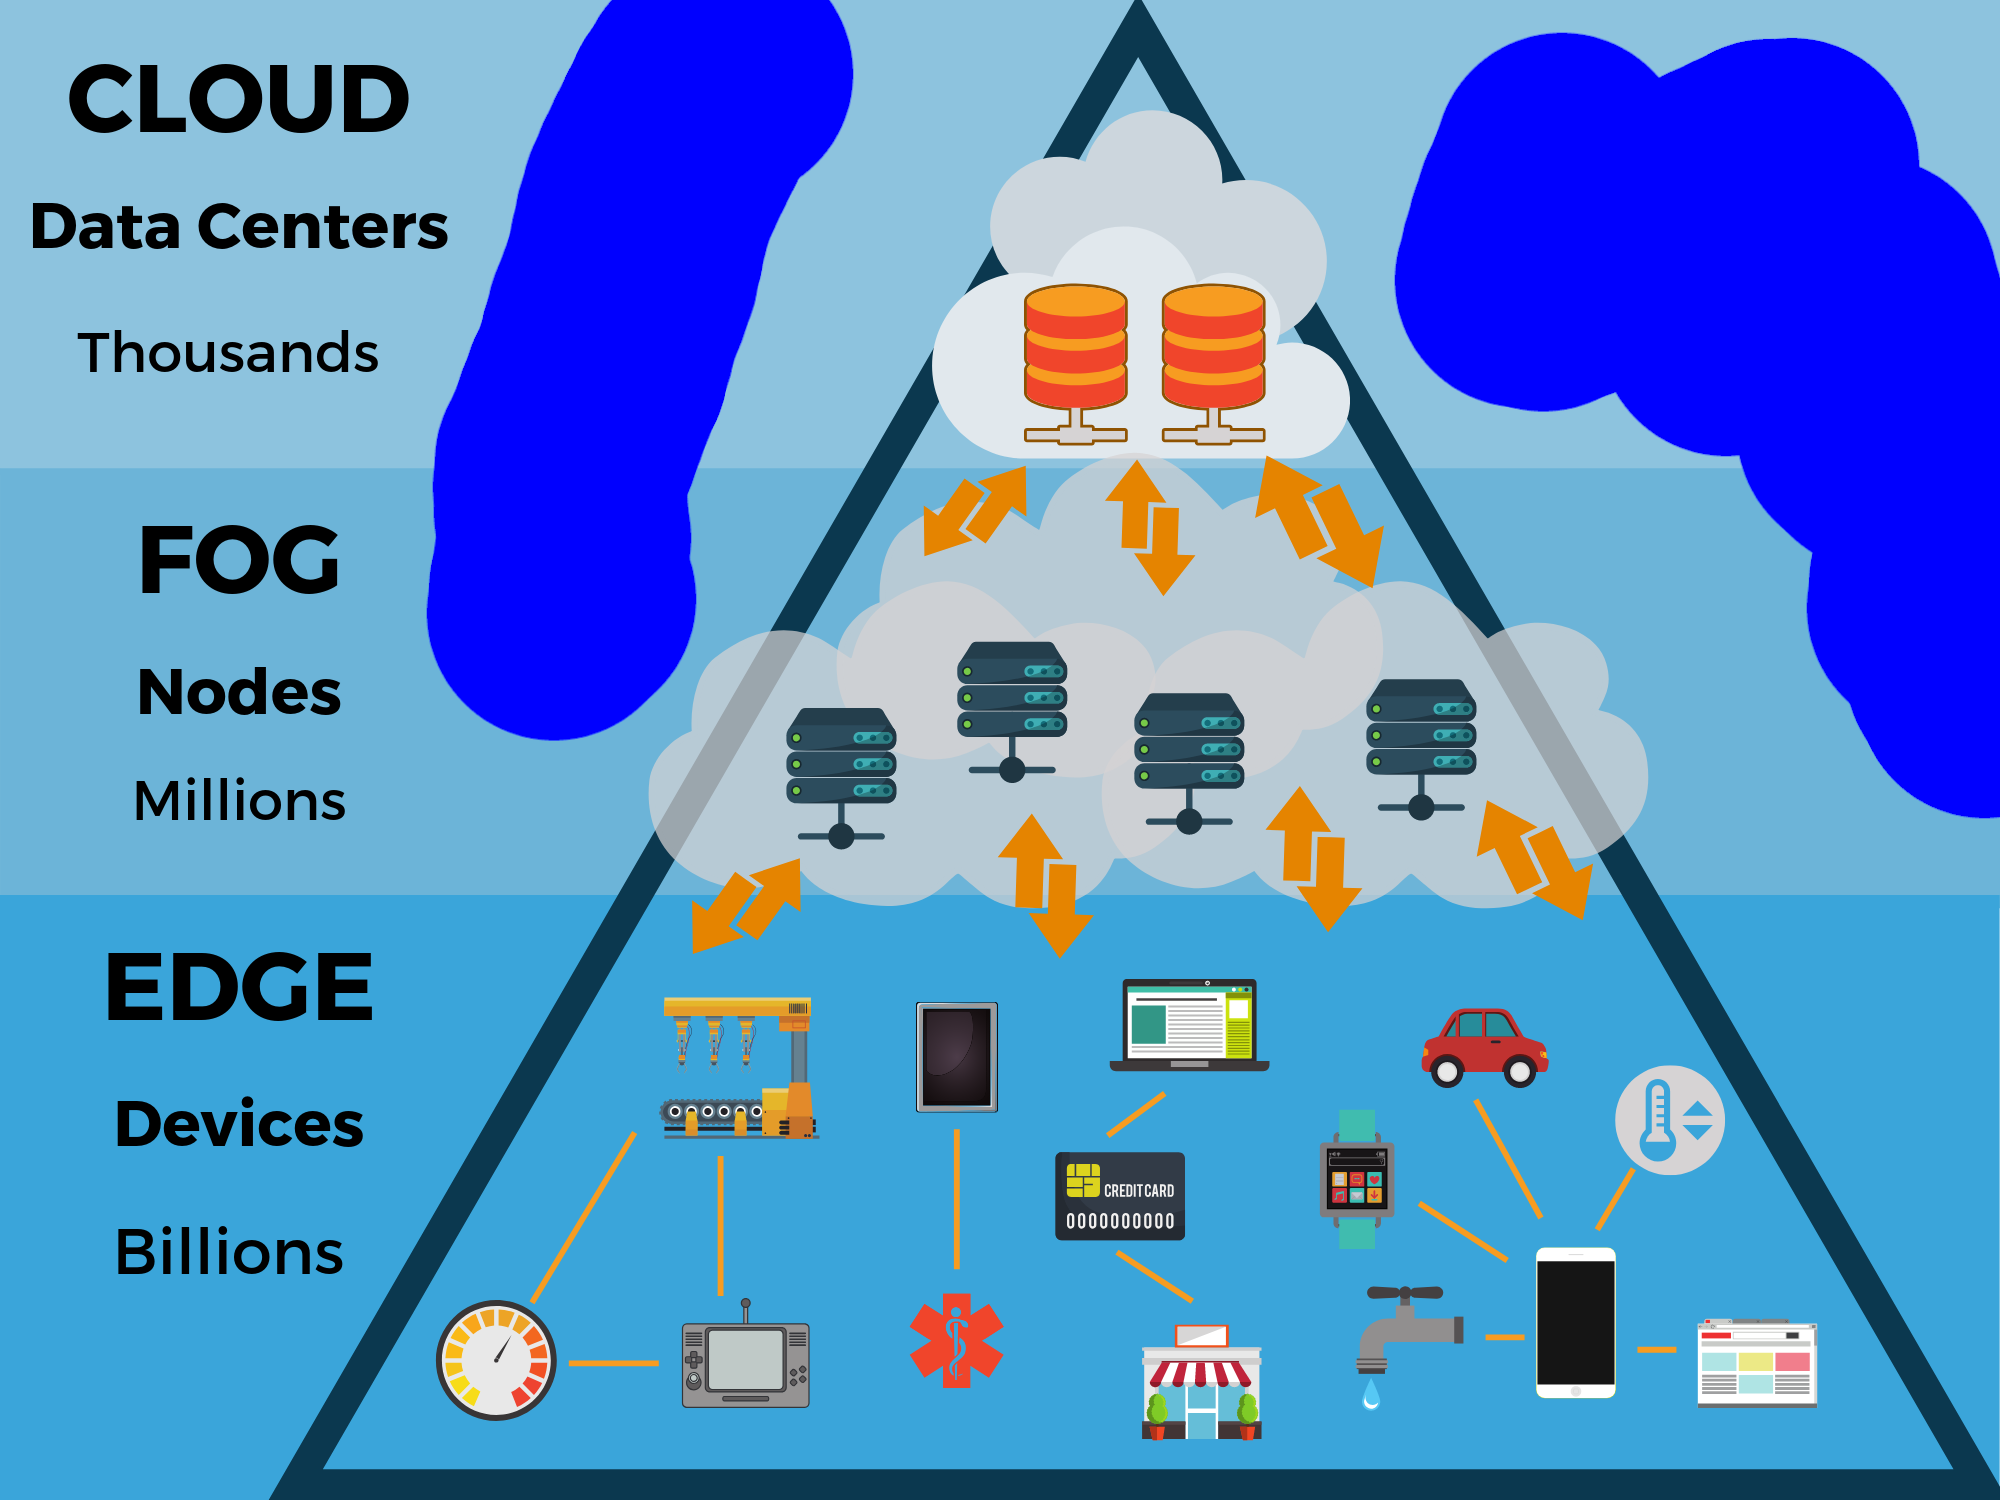
\includegraphics[width=0.75\textwidth]{resources/img/computing_paradigms.png}\\
			\caption{Edge, Fog and Cloud Computing}
			\label{computing_paradigms}
		\end{figure}
	
		% TODO spiegare meglio
		Each of these, places the computation on a different layer of the network, from Cloud Computing that lift off all the need for devices to compute data, to Edge Computing, where there might be specialized servers physically placed in strategic points so that they are closer to the end devices (lower latency), which may even have the ability to compute data by themselves.
		%https://www.cisco.com/c/en/us/solutions/computing/what-is-edge-computing.html
		On the other hand, Fog Computing is less aggressive than Edge Computing, and does not require the same amount of services placed near the clients, but they can be sorted among the backbone of the network.
		
		These communications do not take place only via WiFi or Ethernet.
		Given that ``things'' can be everywhere, the need for a network that can adapt to a fast paced environment is becoming a must.
		Here is where the 5th generation of cellular connectivity comes into play.
		
		%https://www.gsma.com/iot/resources/iot-5g-ltem-nbiot-opportunities-benefits/
		As described in a 2019 whitepaper by GSMA on the IoT and the use of 5G, a ``combination of 5G and wireless edge technologies will support demanding  use cases, such as autonomous driving, time-critical industrial IoT manufacturing processes and  augmented and virtual reality (AR/VR)''\cite{IoT_5g_era}.
		Compared to what is possible with other transmission technologies, 5G supports a massive number in connections, with very little latency.
			
		All of this is not only interesting from a research point of view, but also from a market point of view, where new devices, for consumer and industrial purposes, are created to suit every possible need, that is why IoT can be considered as the ``next chapter of digital communication''.
		
		% TODO riscrivere parlando di health e home automation
		The most notable example from a consumer's point of view, is the smartwatch, which started with the infamous Pebble watch, and is now considered almost a ``must-have'' extension of the smartphone.
		Not only it can be used for recreational purposes, but it is crossing the line to become medical devices, given the improving accuracy with which they record data.
		Data that, in conjunction with AI, can be used to predict heart attacks \cite{7946780} or other diseases, like Hyperkalemia \cite{HYPERKALEMIA}.
		Even now IoT devices and frameworks can be used for contact tracing in order to prevent the spread of Covid-19 \cite{9181512}.
		% Although, it is important to notice that not all projects have succeed, smart glasses by google
		
%		Home automation is another big market
%		Consumers want remote control
%		of devices such as coffee pots so that they may wake up to freshly
%		brewed coffee, or cause coffee to be prepared at a precise time after
%		the completion of dinner preparations.
%		\footnote{\textit{Hyper Text Coffee Pot Control Protocol}: \url{https://datatracker.ietf.org/doc/html/rfc2324}}
		
		On the other hand, from an industrial point of view, there are 
		
		\vspace{3cm}
		
		
		The more data available, the more there are opportunities for science, services, business etc. to understand and grow.
		
		IoT is an enabler for the sciences that need large amount of data for creating algorithms and offering better services and more well tailored products.
		% https://www.siemens-advanta.com/blog/what-are-expected-iot-trends-2021
		
		Another important definition of IoT is IIoT, which stands for Industri 4.0 IoT.
		
		Given the importance of this economic sector, many companies, both technical and not, have analyzed the trends and have been producing forecasts about the growth of IoT.
		% measure commercial adoption of the then-emerging technology. 
		
		One analysis, made by The Economist's Intelligence Unit, and sponsored by Arm \footnote{\url{https://www.arm.com/}}, states that ``More than two-thirds of respondents agree that understanding the value of data helps them articulate the business case for IoT investments.''\cite{economist-iot-business-index-2020-arm}.
		In the same analysis, has emerged that IoT is an enabler for AI, since many companies ``view IoT and AI as two components of an advanced analytics capability''.
		
		But there is more to the IoT than consumer devices
		
		In my opinion, it is important to understand the growth of IoT not only from an academic perspective, but from an economic perspective as well, since today's academic discoveries should be 
			
		Underlying hardware challenges such as battery development and energy retention and consumption are among the main research areas that are being investigated, since they represent challenges to the realization of efficient IoT systems.
		
		

\newpage
\section{Air quality}

% Describe the problem with air quality, link some papers that show that it has been getting worse in the last decades
% Show that there are standards to measure air quality		
% Say something about air quality in the covid era (covid has helped people re-evaluate the use of bikes and other publicly-shared methods of transportation)
% Stopping, although painful for the society (physically and economically) has helped demonstrating that there is still hope to get a clean environment in which to live


% https://www.history.com/news/keeling-curve-global-warming-climate-change

% https://milano.corriere.it/notizie/cronaca/20_maggio_29/inquinamento-quali-sono-effetti-lockdown-zaino-studia-l-aria-milano-13-citta-mondo-50c721a6-a0d4-11ea-bedb-9a92490f6ea3.shtml
% https://www.rinnovabili.it/ambiente/biella-zaino-misura-smog-654/

\newpage
\section{iot for sensing of air quality}

\newpage
\section{MegaSense}

	MegaSense, developed at the University of Helsinki's department of Computer Science\footnote{text}

	\subsection{Hope}